%
% 2dvariation.tex -- zweidimensionale Variation
%
% (c) 2021 Prof Dr Andreas Müller, OST Ostschweizer Fachhochschule
%
\bgroup
\definecolor{hellrot}{rgb}{1.0,0.4,0.8}
\definecolor{hellblau}{rgb}{0.2,0.6,0.6}
\begin{frame}[t]
\setlength{\abovedisplayskip}{5pt}
\setlength{\belowdisplayskip}{5pt}
\frametitle{Variation in 2D}
\vspace*{-10pt}
\begin{center}
\begin{tikzpicture}[>=latex,thick]
\coordinate (L) at (-0.55,0.9);
\coordinate (V) at (-1.5,2.7);


\only<1>{
\node at (0,0) {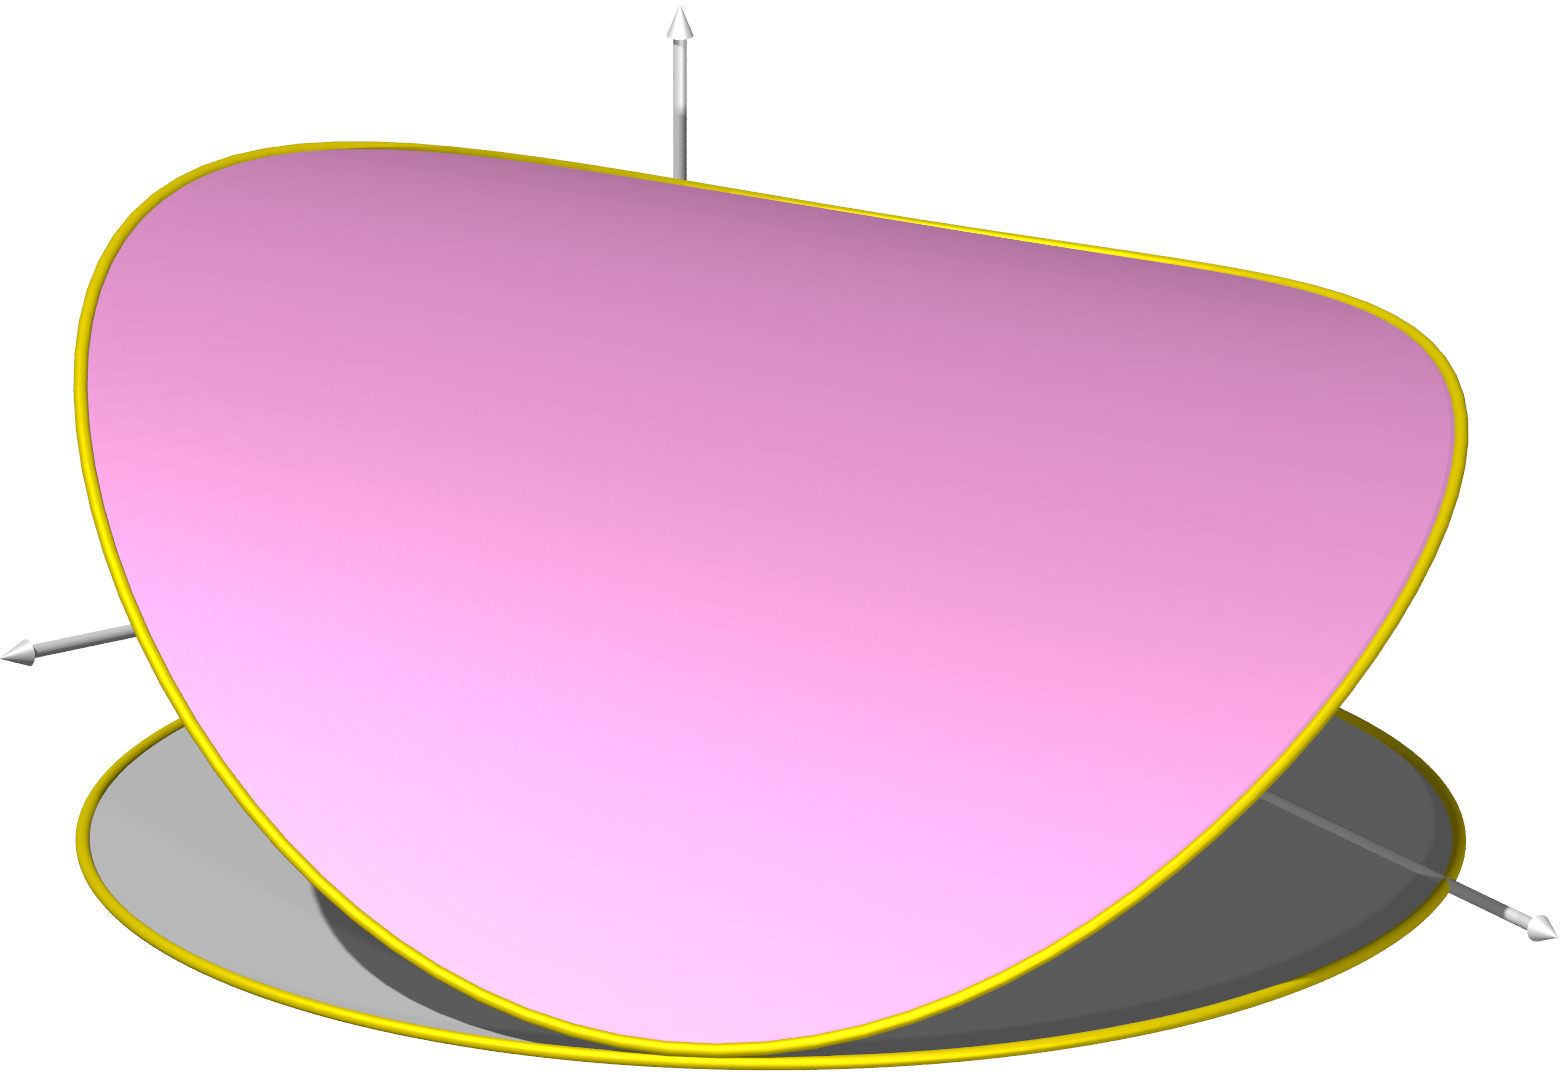
\includegraphics[width=11cm]{../../buch/chapters/040-felder/images/flaeche.jpg}};
}

\uncover<2->{
\node at (0,0) {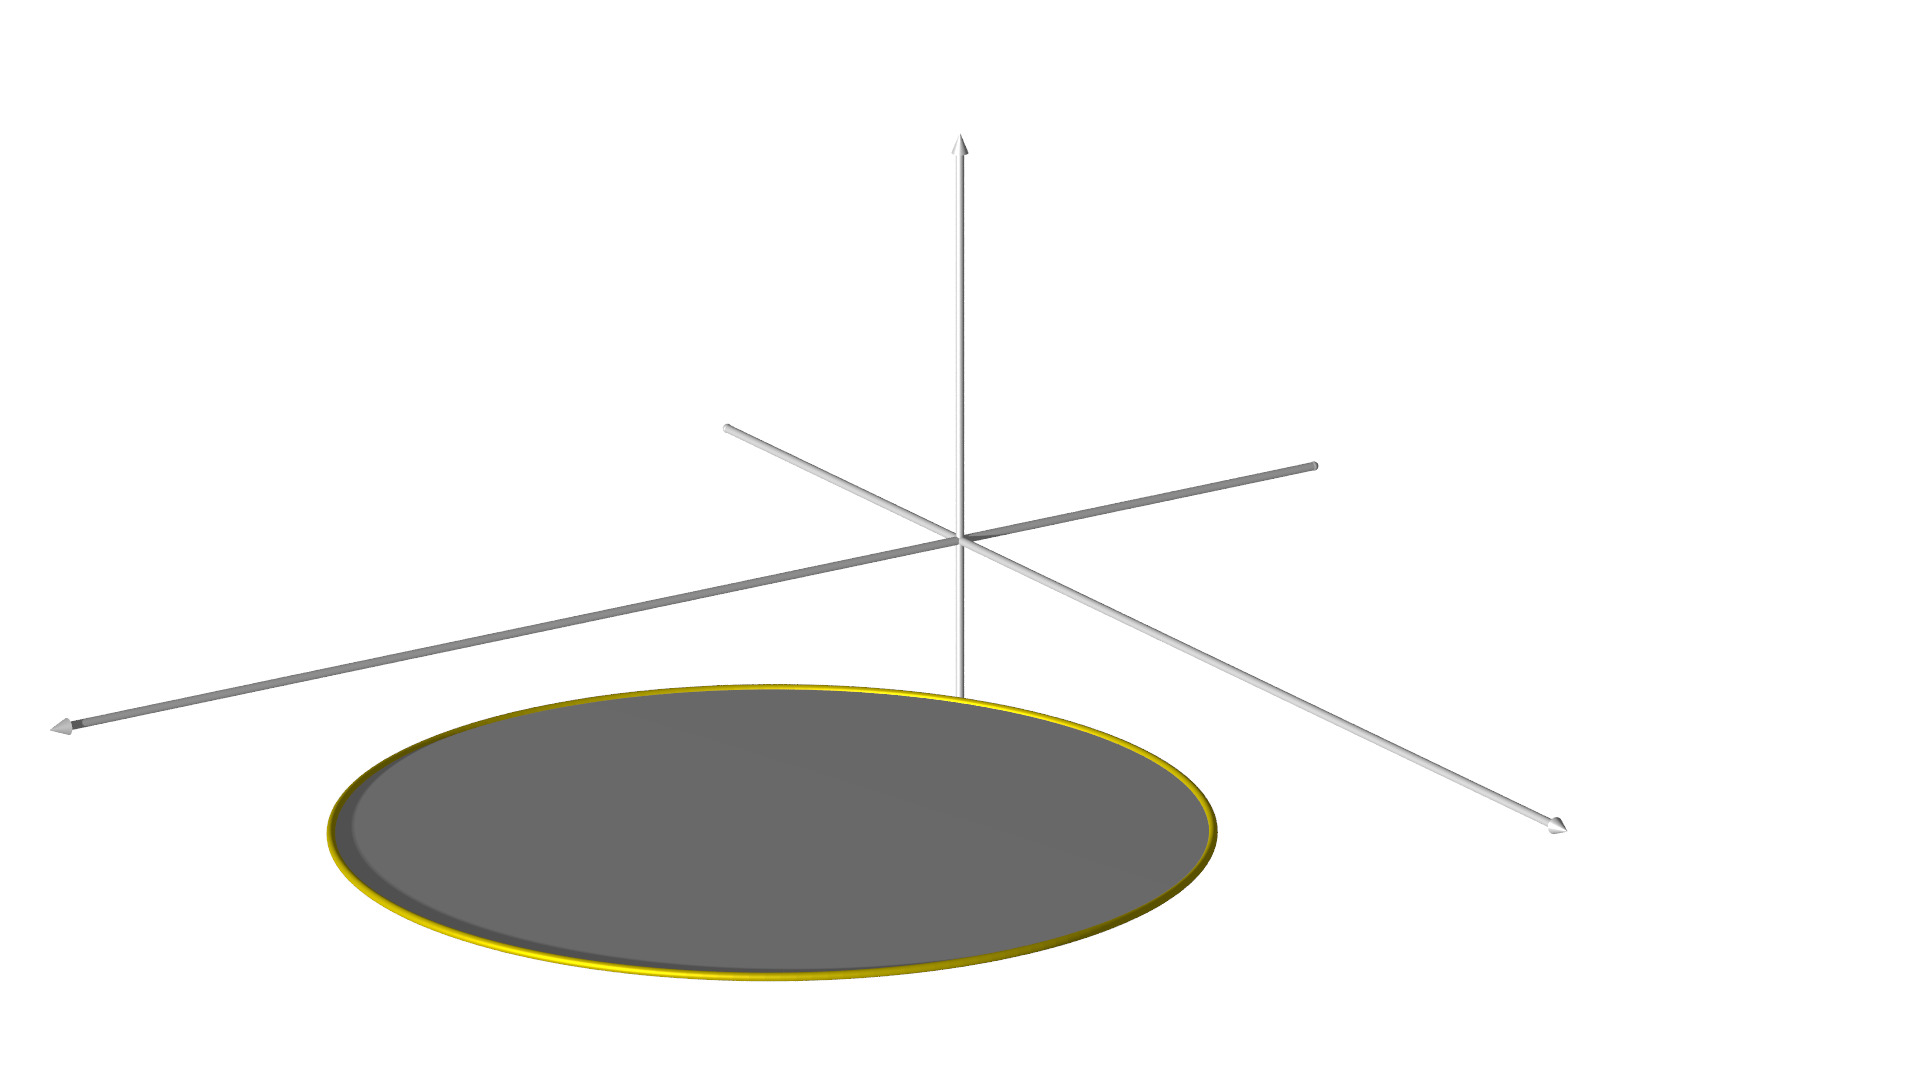
\includegraphics[width=11cm]{../../buch/chapters/040-felder/images/variation.jpg}};
%\node at (-0.4,-2.8) {$\Omega$};
}

\uncover<1,3->{
	\fill[color=white,opacity=0.7] ($(L)-(1.0,0.25)$) rectangle +(2.0,0.5);
	\node[color=hellrot] at (L) {$z=u(x,y)\mathstrut$};
}

\uncover<4->{
	\fill[color=white,opacity=0.7] ($(V)-(1.9,0.25)$) rectangle +(3.8,0.5);
	\node at (V) {$z = {\color{hellrot}u(x,y)} + \varepsilon{\color{hellblau}\eta(x,y)}\mathstrut$};
}

\node at (-4.2,-2.2) {$\Omega\mathstrut$};

\node at (-5.3,-0.55) {$x\mathstrut$};
\node at (5.5,-2.4) {$y\mathstrut$};
\node at (-0.45,3.7) {$z\mathstrut$};
\end{tikzpicture}
\end{center}
\end{frame}
\egroup
